\documentclass[smaller]{beamer}
\usepackage{beamerarticle}
\mode<presentation> {
  \usetheme{Montpellier}
  \useinnertheme{circles}
  \usecolortheme{sidebartab}
  \setbeamercolor{structure}{fg=blue}
  % or ...

%  \setbeamercovered{transparent}
  % or whatever (possibly just delete it)
}
\usepackage{movie15}
\usepackage[utf8]{inputenc}

\usepackage[english,russian]{babel}
\usepackage{listings}
\usepackage[T2A]{fontenc}
%\usepackage{amssymb,amsmath,mathrsfs,amsthm}

\usepackage[footnotesize]{caption2}
\usepackage{indentfirst}
\usepackage{multicol}
%\usepackage[cp1251]{inputenc}
% %\usepackage[russian]{babel}
\usepackage{amssymb,amsmath}

%\usepackage[T2A]{fontenc}
\usepackage[utf8]{inputenc}
\usepackage{graphicx, graphics, epsfig}
\usepackage{epstopdf}
\usepackage{ifpdf}  
%\usepackage[scaled=.92]{helvet}
%\usepackage{times}
\usepackage{mathrsfs}
\usepackage{amsfonts}
\usepackage{floatflt}

%\usepackage[pdftex,unicode]{hyperref}
%\usepackage[cp1251]{inputenc}
%\usepackage[utf8]{inputenc}
%\usepackage{listings}
%\usepackage[pdftex,unicode]{hyperref}
%\usepackage[english]{babel}
%\usefonttheme{serif}
% Or whatever. Note that the encoding and the font should match. If T1
% does not look nice, try deleting the line with the fontenc.


\title[P-Паттерны]{Параллельная реализация метода поиска закономерностей в последовательностях событий} % (optional, use only with long paper titles)

\author % (optional, use only with lots of authors)
[~]{Вишневский В.В.}


\AtBeginSubsection[] {
  \begin{frame}<beamer>
    \frametitle{Plan}
    \tableofcontents[currentsection,currentsubsection]
  \end{frame}
}
\begin{document}

\begin{frame}
  \titlepage
\end{frame}

%\begin{frame}
 % \frametitle{План}
 % \tableofcontents
  % You might wish to add the option [pausesections]
%\end{frame}



\section{Исследование поведения}

\begin{frame}	
  \frametitle{Задача исследования поведения}
В поведении существуют закономерности. Повседневные
церемонии: ритуалы приветствия, рабочие процессы, груминг у животных,
состоят из поведенческих паттернов.
\\~\\

Пример. Принятие пищи: <<подойти к столу>>, 
<<отодвинуть стул>>, <<сесть>>, <<съесть главное блюдо>>, 
<<съесть десерт>>, <<выпить чай>>, <<отодвинуть стул>>,
<<встать>>, <<отойти от стола>>.
%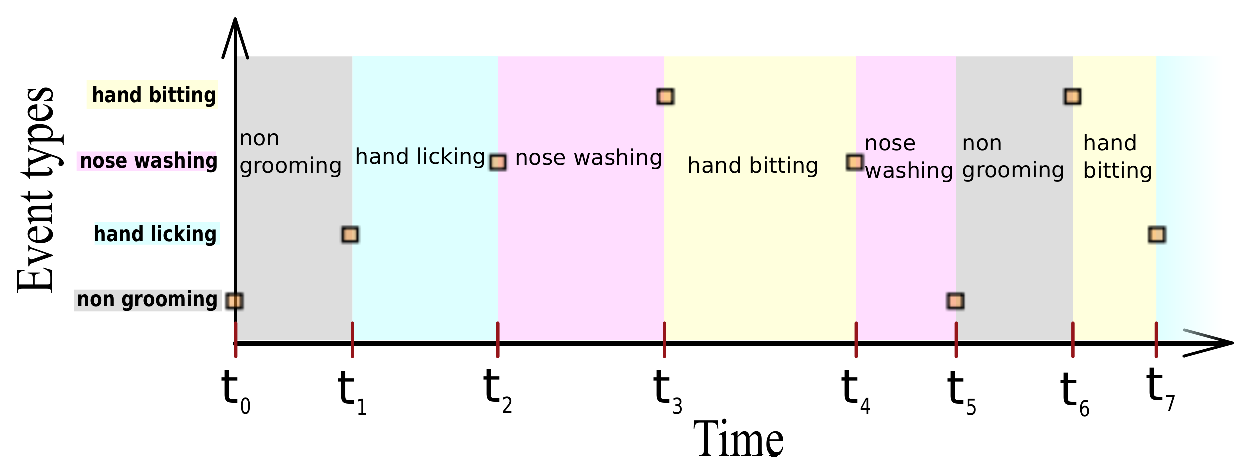
\includegraphics[scale=0.40]{beh_data.eps}

\begin{itemize}
 \item События связанны временн\'{ы}ми интервалами.
 \item Есть иерархия.
\end{itemize}

\end{frame}


\begin{frame}	
  \frametitle{Мотивация}
Выделив такие поведенческие паттерны, становится возможно:
\\~\\
\begin{itemize}
  \item делать выводы о сложности поведения,
  \item определять изменения в поведении наблюдаемых животных,
  \item {\em измерять} поведение~--- анализировать влияние 
	различных факторов на поведение.
\end{itemize}
%\begin{left}
%\begin{tabular}[t]{p{12em}|p{12em}}
%    \includegraphics[scale=0.25]{NEWTS.eps} & 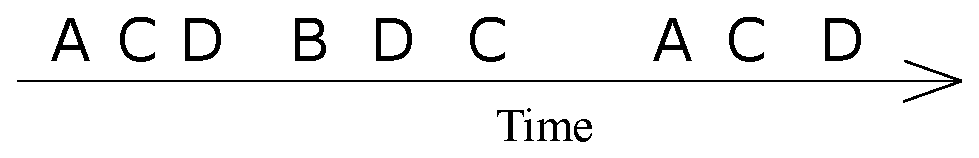
\includegraphics[scale=0.25]{TSNEW2.eps}\\
%\end{tabular}
%\end{left}
\end{frame}

\begin{frame}	
 \frametitle{Входные данные}

%\begin{figure}[ht]
%\includemovie[poster,text={\includegraphics[width=8cm, height=6cm]
%{beh_data.eps}},autoplay,mouse=true]{8cm}{6cm}
%{video_kth.avi}
%\end{figure}
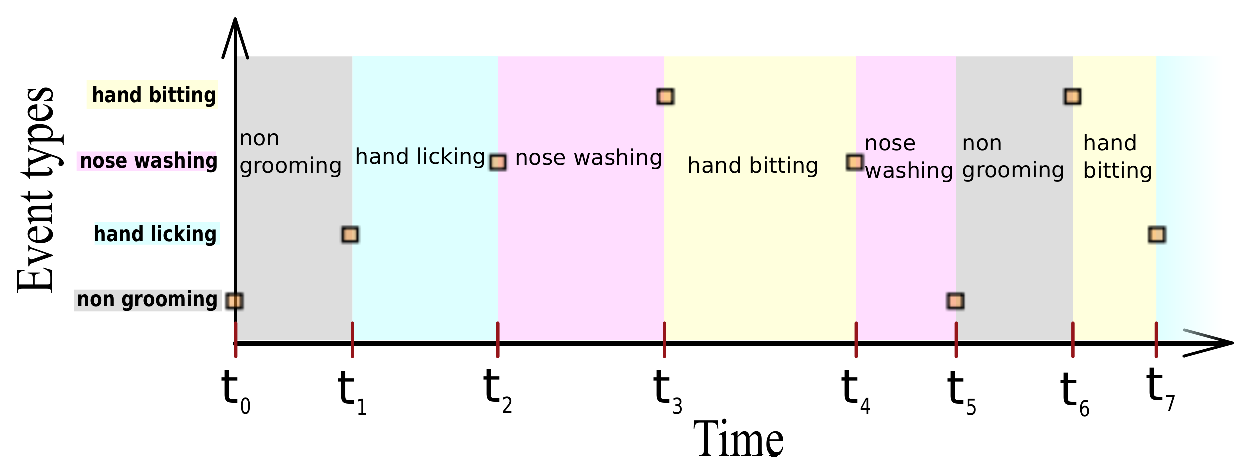
\includegraphics[scale=0.5]{beh_data.eps}
%\begin{figure}[ht]
%\includemovie[
%poster,
%label=cells,
%  text={\small Test mplayer with acroread}
  %mimetype=video/mpg,
%]{12cm}{6cm}{video_kth.avi}
%\end{figure}

  %  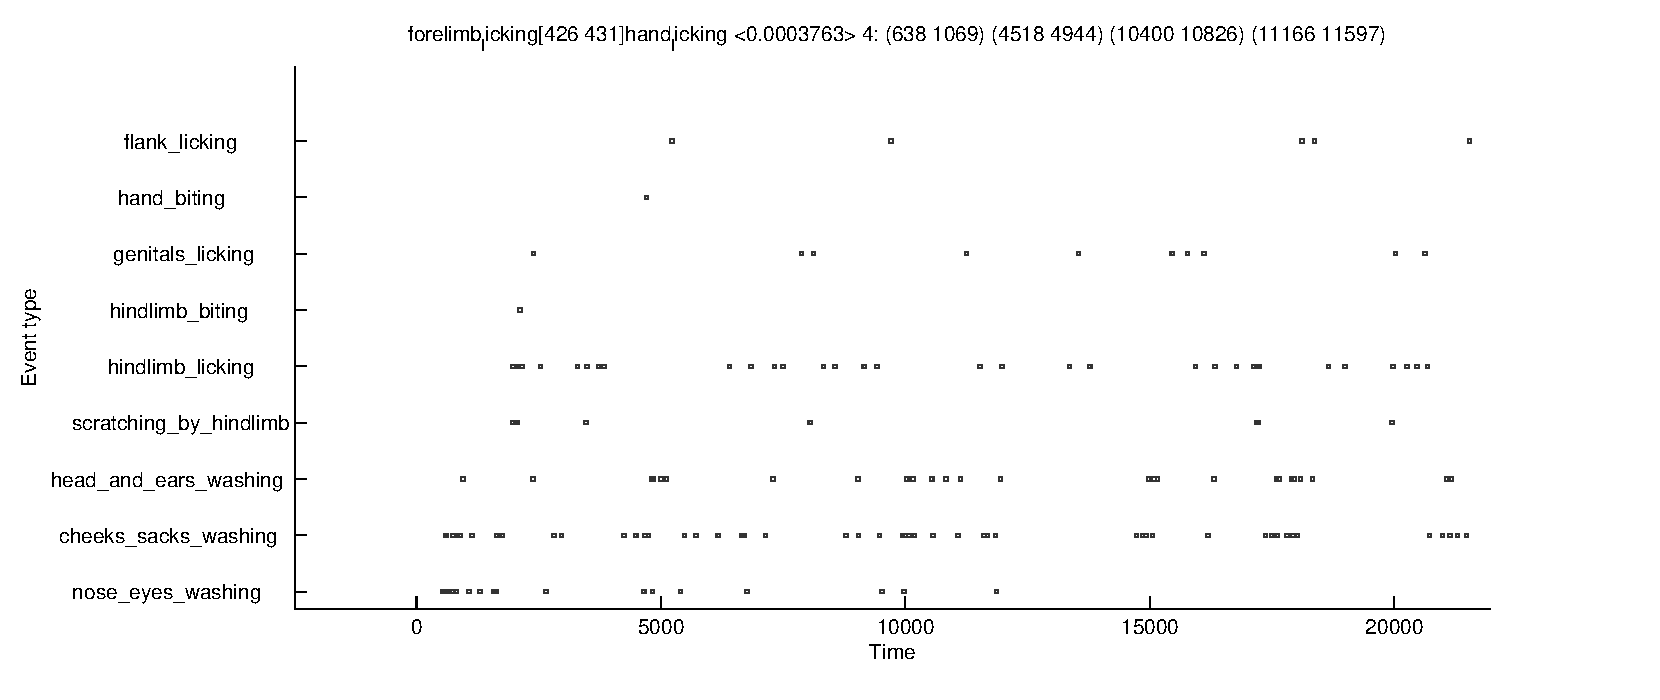
\includegraphics[scale=0.4]{TS.eps} 
\end{frame}

\begin{frame}
  \frametitle{Недостатки существующих методов}
  \begin{itemize}
   \item Стандартные методы поиска закономерностей не предназначены для поиска {\em поведенческих} паттернов
    (важна иерархия, упорядоченность, временн\'{ы}е интервалы).
   \item Существуют методы поиска закономерностей, где учитывается только порядок актов.
   \item Широко используемый метод поиска Т-Паттернов {\bf очень} чувствителен к шуму, допускает слабую \emph{вариабельность} паттернов. 
      Закрытые исходные коды.
  \end{itemize}
\end{frame}


\begin{frame}	
  \frametitle{Подход к поиску паттернов}
Паттерн~--- это часто встречающаяся последовательность событий(поведенческих актов), возникающих один за другим 
через определенные промежутки времени.
\\~\\
  Инициализируем множество паттернов поведенческими актами. Потом итеративно повторяем:
  \begin{itemize}
   \item {\bf Конструирование:}Для всех пар паттернов проверить, повторяется ли один за другим достаточно часто. Если да, 
	то получаем новый паттерн. 
   \item {\bf Редукция:} Удалить одинаковые паттерны, которые были сконструированы по-разному.
  \end{itemize}
\end{frame}

\subsection{P-Паттерны}
\begin{frame}
\frametitle{Вероятностная модель P-Паттерна}
 \begin{itemize}
  \item $P=A[\mu_A,\sigma_A]B[\mu_B,\sigma_B]C[\mu_C,\sigma_C]$\\
 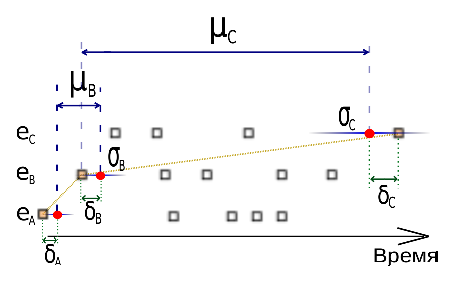
\includegraphics[scale=0.6]{il1.eps} \\
  \item Функция потерь:
        $$
  f_{LOSS}(x,N)= \begin{cases}
   \exp\bigl(-\frac{\lambda x}{N}\bigr), & x < N, \\
   0,                                    & x=N.
   \end{cases}
  $$
  \item Правдоподобие паттерна:
$$L_{P}(\varepsilon)=
f_{LOSS}(N_-,N_{P})
\prod_{i=1}^{N_{P}}\left( \frac1{\sqrt{2\pi}\,\sigma_i }\right) 
\prod_{i\in \mathcal{N}_+}\exp\left(- \frac{\delta_i^2}{2\sigma_i^2}\right) 
$$
 \end{itemize}
\end{frame}  

\begin{frame}
\frametitle{Правдоподобие}
\begin{figure}[H]
\noindent\centering{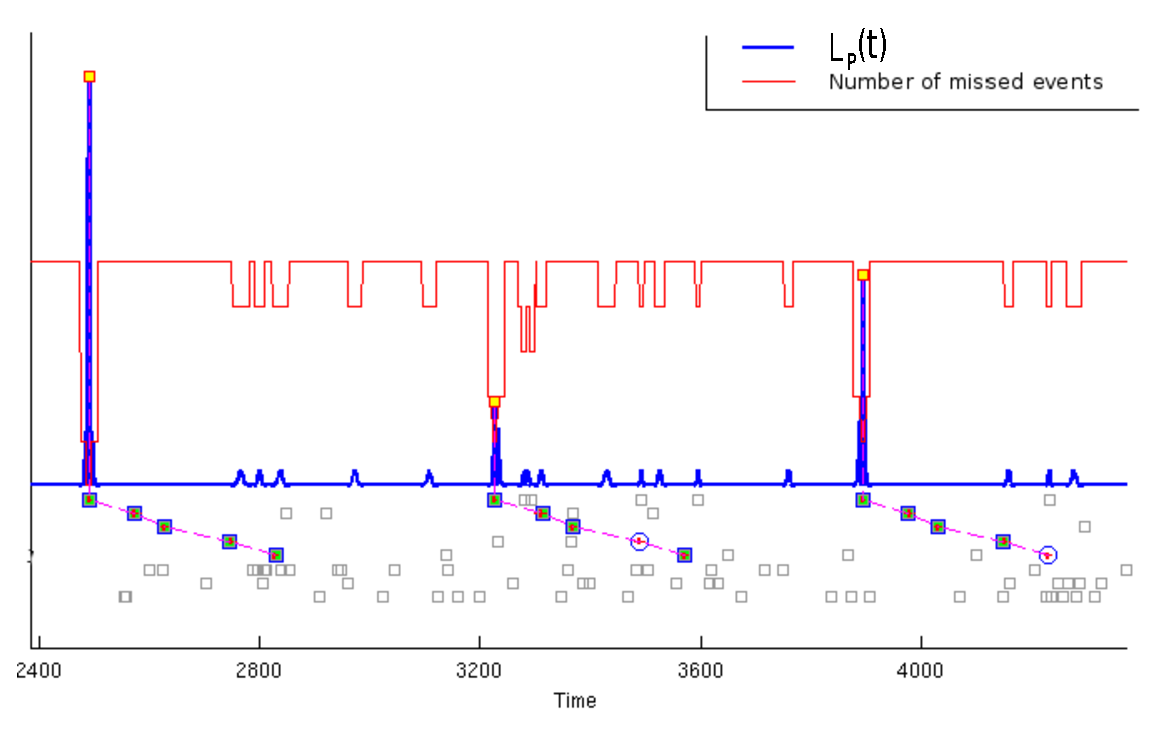
\includegraphics[scale=0.4]{norm_12_of_14.eps}}
\caption{ Пример функции правдоподобия паттерна. Желтыми маркерами с красной границей изображены максимумы функции правдоподобия: 
моменты времени, когда мы считаем, что паттерн имеет место.
В нижней части рисунка закрашенными квадратами показаны присутствующие
события, полыми кружками~--- пропущенные события в паттерне. Полые серые квадраты соответствуют наблюдаемым поведенческим актам.}
\end{figure}
\end{frame}  

% \begin{frame}
%   \frametitle{ Параметры предложенного метода }
%     {\small
%    \begin{tabular}{|p{2em} | p{5em} | p{3em} | p{12em}| }
%     \hline
%     \bf{Пар-р} & \bf{ Возможные\newline значения} & \bf{ defaults } &\bf{ На что влияет } \\
%     \hline\hline
%     \centering$\alpha$   & \centering$[\,0, 1]$ & \centering $0.001$ & Уровень значимости паттерна \\ \hline
%     \centering$N_{min}$ &  \centering$[\,0, +\infty]$ & \centering 3 & Минимальное количество появлений паттерна в данных  \\ \hline 
%     \centering$\lambda$  & \centering$[\,0, +\infty]$ & \centering 8 & Допустимая степень нечеткости паттерна  \\  \hline    
%     \centering$\nu$      & \centering$[\,0, 1]$ & \centering 0.6 & Минимальная степень похожести паттернов для удаления \\ \hline
%     \centering$\gamma$   & \centering$[\,0, 1]$ & \centering 0.4 & Чувствительность к отклонению от ожидаемого правдоподобия \\ \hline
% \end{tabular}}
% 
% \end{frame}


\section{Параллельная реализация}
\begin{frame}
  \frametitle{Т-Паттерны и P-Паттерны}
  \begin{itemize}
   \item T-Паттерны распараллеливаем на SMP с помощью OpenMP. Тестирование на 4-х ядерном CPU. Примерная сложность: $O(n^2)$.
  \item P-Паттерны распараллеливаем на GPU с помощью CUDA. Тестирование на GF 8800GTX, 128 потоковых процессора. Примерная сложность: $O(n^3)$.
  \end{itemize}
\end{frame}

\begin{frame}
 \frametitle{Ускорение OpenMP}
\begin{figure}[H]
\centering{	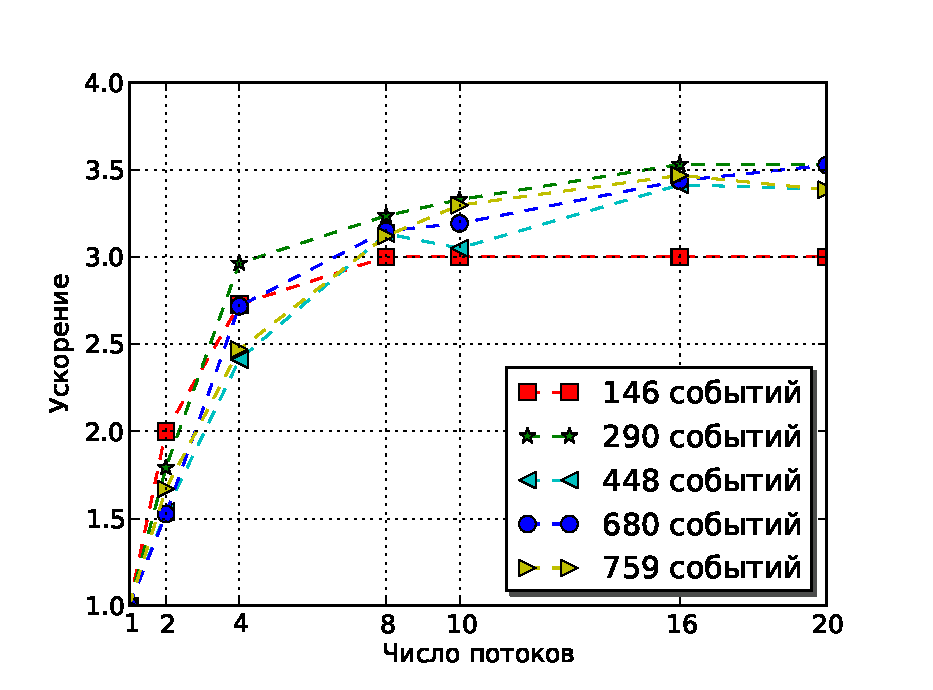
\includegraphics[scale=0.5]{omp_su.eps} }
	\caption{Ускорение алгоритма поиска Т-Паттернов на 4-х ядерном процессоре.}
\end{figure}
    
\end{frame}


\begin{frame}
  \frametitle{Ускорение алгоритма поиска P-Паттернов. CUDA}
\begin{figure}[H]
\centering{	\includegraphics[scale=0.45]{cuL_su.eps} }
	\caption{Ускорение стадии подсчета правдоподобия паттернов в зависимости от размера входных данных.}
\end{figure}

\end{frame}

\begin{frame}
  \frametitle{Ускорение алгоритма поиска P-Паттернов. CUDA}
\begin{figure}[H]
\centering{	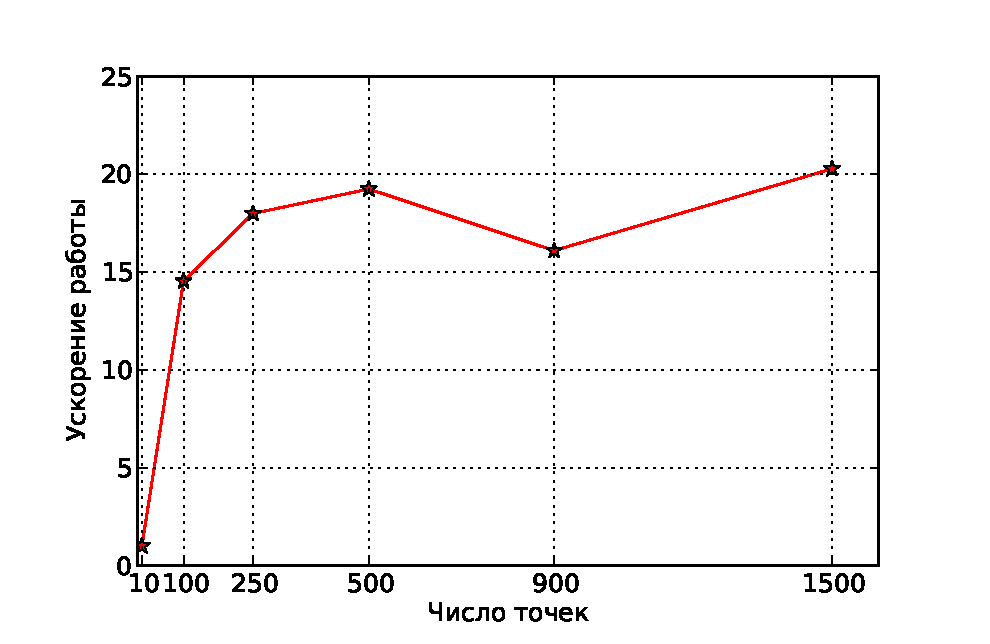
\includegraphics[scale=0.3]{cuD_su.eps} }
	\caption{Ускорение стадии конструирования паттернов в зависимости от размера входных данных.}
\end{figure}

Ускорение метода в целом $\sim$ 40 раз. \\
Типичные экспериментальные данные: 12 секунд на GPU, 470 секунд на CPU(1 поток).\\
Утилизация GPU $\sim$ 230 GFLOPS (Заявленная производительность 518 GFLOPS)

\end{frame}


\section{Эксперимент на реальных данных}

\begin{frame}
  \frametitle{Эксперимент с грызунами без гиппокампа}
  \begin{itemize}
   \item Гиппокамп~--- отдел головного мозга. Его функции 
связывают с механизмами работы памяти, обучением, пространственной
навигацией.
   \item Две группы: контрольная(12 особей) и грызуны без гиппокампа(12 особей).
   \item Определить по поведению к какой группе относится особь.
   \item Как меняется поведение после воздействия на определенный участок мозга?
  \end{itemize}
\begin{figure}[H]
\centering{	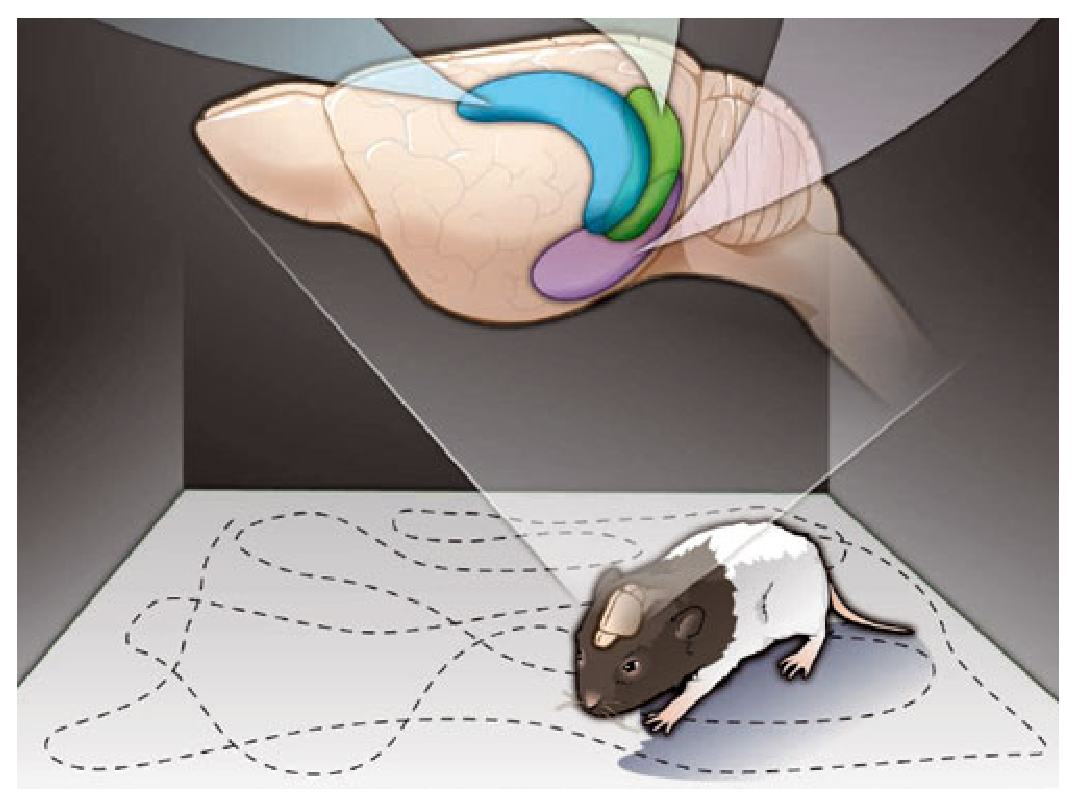
\includegraphics[scale=0.3]{hippocamp.eps} }
\end{figure}
\end{frame}

\begin{frame}
  \frametitle{Результаты экспериментов}
\begin{figure}[H]
\noindent\centering{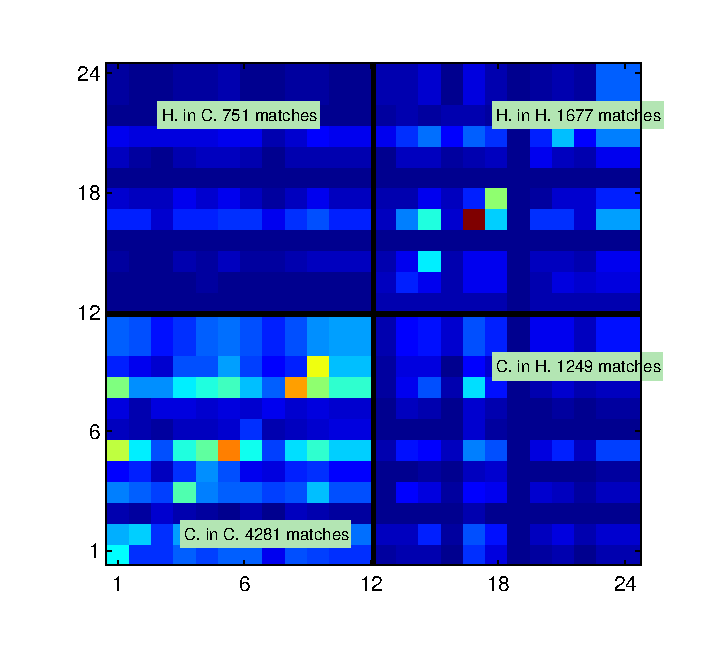
\includegraphics[scale=0.5]{cross_m_big.eps}}
\caption{ Таблица соответствий паттернов. Неформально: 
по вертикали {\em откуда} берутся паттерны, по горизонтали~--- {\em где} ищутся вхождения этих паттернов; например, в ячейке $(3,10)$ записано
число соответствий паттернов третей особи в поведении десятой.}

\end{figure}
\end{frame}

\begin{frame}
  \frametitle{Результаты экспериментов}
\begin{figure}[H]
\noindent\centering{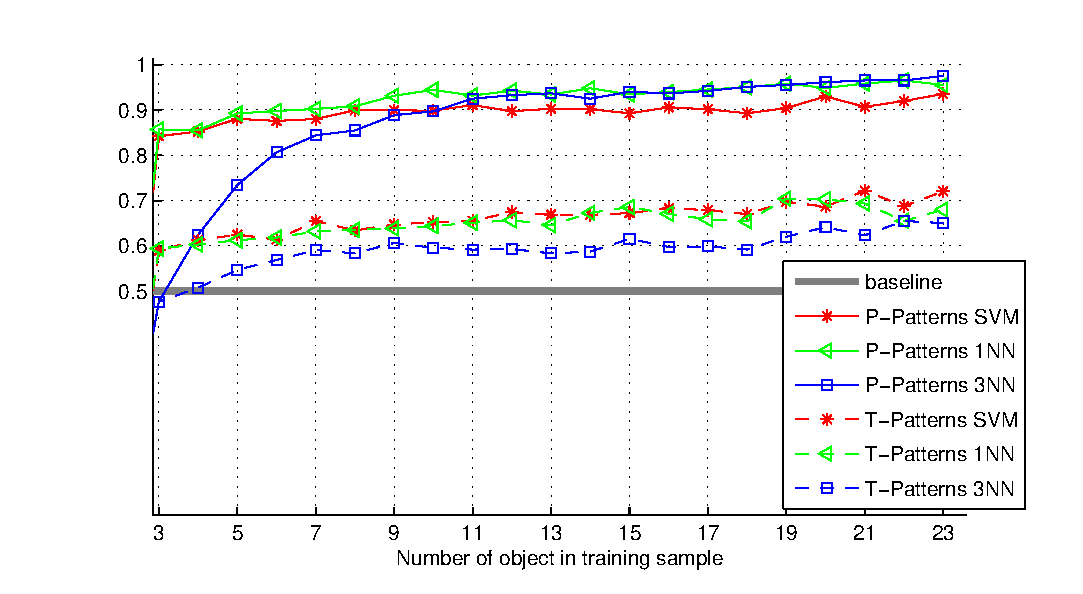
\includegraphics[scale=0.5]{2classes.eps}}
\caption{ Средняя доля правильных ответов классификации методами SVM и $k$NN с разными способами поиска паттернов, в зависимости от размера
обучающей выборки. Средняя доля правильных классификации: P-Паттерны~--- 92\%, Т-Паттерны~---68\%.  }
\end{figure}
\end{frame}

\begin{frame}
  \frametitle{Характерные классу животных паттерны}

\begin{figure}[H]
\noindent
	\begin{multicols}{2}
	\hfill
  \noindent
	\includegraphics[width=55mm]{char_pat.eps}
\vfill\hfill
	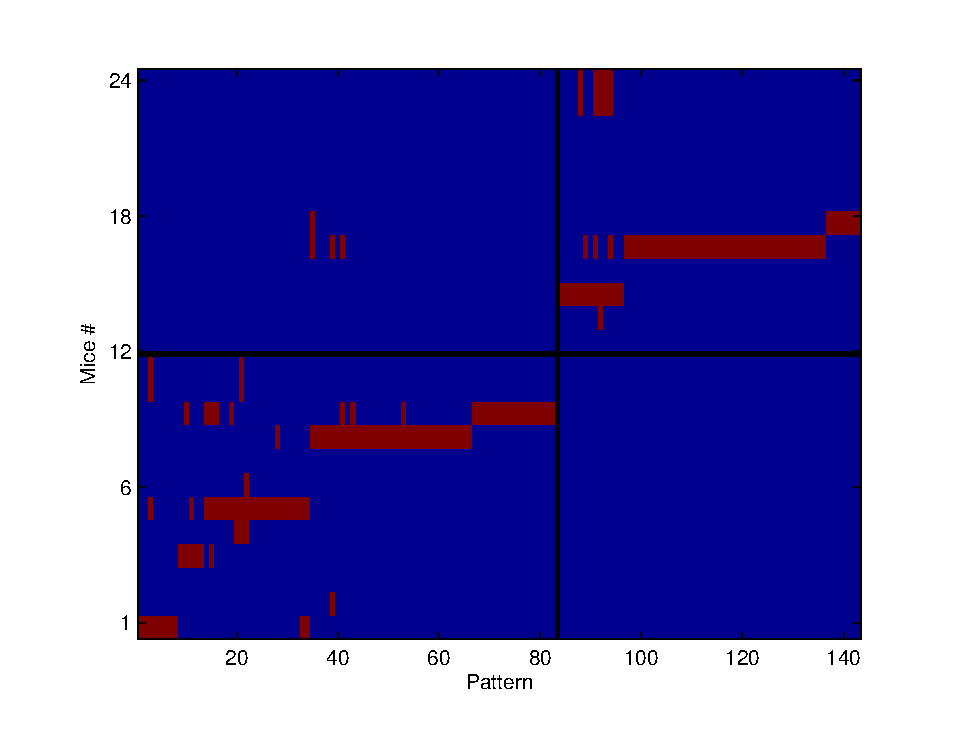
\includegraphics[width=55mm]{char_tpat.eps}
	\end{multicols}
	\caption{Встречаемость найденных паттернов в разных группах мышей. Слева изображены P"=Паттерны, справа~--- Т"=Паттерны. Ячейка закрашена красным цветом,
если данный паттерн встретился в поведении определенной особи, иначе ячейка закрашена синим.}
\end{figure}
\end{frame}

\begin{frame}
  \frametitle{Пример характерного P"=Паттерна}
P-Паттерн в формате: <$\dots\text{Событие}_i[\,\mu_i; \sigma_i]$\dots> \quad Смещения даны в секундах .
\\ ~\\ \begin{center}
\line(1,0){250}
\end{center}
 Вычес-е задн. конечностями $[22.9;\; 7.9]$
 Вылиз-е ладоней $[1.1;\; 2.7]$
 Быстр. умыв-е носа $[0.4;\; 0.5]$
 Умыв-е головы с ушами $[ 3.2;\; 7.9 ]$
 Умыв-е носа $[ 17.0;\; 7.9 ]$
 Вылиз-е задн. конечностей
 \\ \begin{center}
\line(1,0){250}
\end{center} ~\\

 Найден у 8 из 12 особей контрольной группы и ни разу не найден в гиппокампальной группе. Имеет биологический смысл.
\end{frame}

\begin{frame}
  \frametitle{Отклик на P-Паттерн в контрольной группе}
\begin{figure}[h]
\noindent\centering{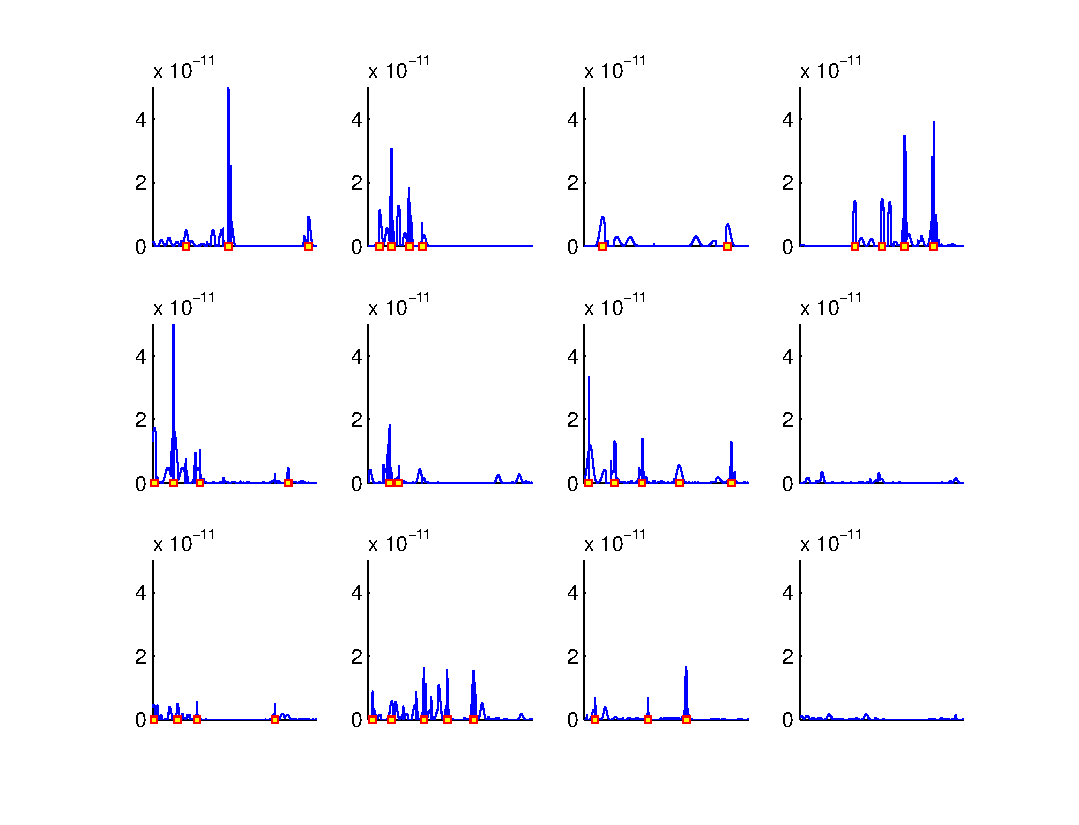
\includegraphics[width=93mm]{patLH_contr.eps}}
\end{figure}
\end{frame}

\begin{frame}
  \frametitle{Отклик на P-Паттерн в гиппокампальной группе}
\begin{figure}[h]
\noindent\centering{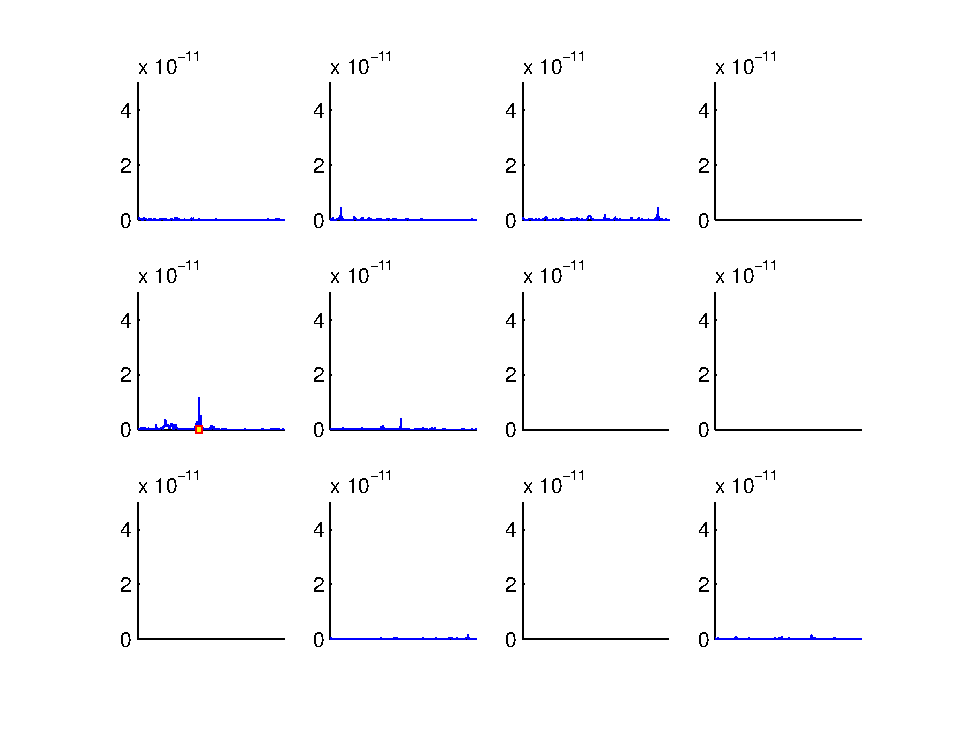
\includegraphics[width=93mm]{patLH_hip.eps}}
\end{figure}
\end{frame}


\section{Заключение}
\begin{frame}
  \frametitle{Выводы}
  \begin{itemize}
   \item Предложенный метод расширяет существующий подход
	  к поиску паттернов.
   \item Устойчивость к шуму.
   \item Более вариабельные паттерны, новый подход к описанию поведения с помощью откликов на множество P"=Паттернов(мешок слов).
   \item Достигнуто ускорение параллельной версии на GPU в 40 раз.
   \item Качество классификации на экспериментальных данных $\sim$ 92\%.
   \item Предложенный метод применим не только для анализа поведения животных(структура ДНК, спайковая активность нейронов, рынки, новостные тренды).

\item[$-$] Сложности на очень маленьких объемах данных.
\item[$-$] Долгое время работы на очень больших объемах данных.
  \end{itemize}
\end{frame}

\begin{frame}
  \frametitle{Выносится на защиту:}
  \begin{itemize}
   \item Разработан новый метод поиска поведенческих закономерностей.
   \item Потенциально новый подход к исследованию поведения.
   \item Создана свободная, документированная, параллельная(ускорение порядка 40 раз) реализация метода.
   \item На реальных данных получен биологический результат: классификация мышей по поведению(качество классификации порядка 92\%).
  \end{itemize}
\end{frame}

\end{document}

